\documentclass[ignorenonframetext, professionalfonts, hyperref={pdftex, unicode}]{beamer}

\usetheme{Copenhagen}
\usecolortheme{wolverine}

\usepackage[orientation=landscape, size=custom, width=16, height=9.75, scale=0.5]{beamerposter}	

%Packages to be included

\usepackage{textcomp}

\usepackage[russian]{babel}
\usepackage[utf8]{inputenc}
\usepackage[T1]{fontenc}

\usepackage{beamerthemesplit}

\usepackage{ulem}

\usepackage{verbatim}

\usepackage{ucs}
\usepackage{listings}
\lstloadlanguages{C, make, bash}

\lstset{escapechar=`,
	extendedchars=false,
	language=C, 
	tabsize=2, 
	columns=fullflexible, 
%	basicstyle=\scriptsize,
	keywordstyle=\color{blue}, 
	commentstyle=\itshape\color{brown},
%	identifierstyle=\ttfamily, 
	stringstyle=\mdseries\color{green}, 
	showstringspaces=false, 
	numbers=left, 
	numberstyle=\tiny, 
	breaklines=true, 
	inputencoding=utf8x,
	keepspaces=true,
	morekeywords={u\_short, u\_char, u\_long, in\_addr}
	}

\definecolor{darkgreen}{cmyk}{0.7, 0, 1, 0.5}

\lstdefinelanguage{diff}
{
    morekeywords={+, -},
    sensitive=false,
    morecomment=[l]{//},
    morecomment=[s]{/*}{*/},
    morecomment=[l][\color{darkgreen}]{+},
    morecomment=[l][\color{red}]{-},
    morestring=[b]",
}



%%%%%%%%%%%%%%%%%%%%%%%%%%%%%%%%%%%%%%%%%%%%%%%%%
%%%%%%%%%% PDF meta data inserted here %%%%%%%%%%
%%%%%%%%%%%%%%%%%%%%%%%%%%%%%%%%%%%%%%%%%%%%%%%%%
\hypersetup{
	pdftitle={Введение в GNU/Linux},
	pdfauthor={Epam/LLPD}
}





%%%%%% Beamer Theme %%%%%%%%%%%%%

	
\title{Введение в GNU/Linux}
\author{Epam/LLPD}



%%%%%%%%%%%%%%%%%%%%%%%%%%%%%%%%%%%%%%%%%%%%%%%%%
%%%%%%%%%% Begin Document  %%%%%%%%%%%%%%%%%%%%%%
%%%%%%%%%%%%%%%%%%%%%%%%%%%%%%%%%%%%%%%%%%%%%%%%%




\begin{document}

\frame{
	\frametitle{Сетевые интерфейсы Linux}
	\titlepage
	\vspace{-0.5cm}
	\begin{center}
	%\frontpagelogo
	\end{center}
}
\frame{
	\tableofcontents
%	[hideallsubsections]
}

\begin{frame}{Сетевая подсистема Linux}

	\begin{block}{Cетевой интерфейс}

		Сетевой интерфейс в Linux -– это абстрактный именованный объект,  используемый для передачи 
		данных через некоторую линию связи без привязки к ее (линии связи) реализации.
	\end{block}
\end{frame}

\begin{frame}{Сетевая подсистема Linux}

	\center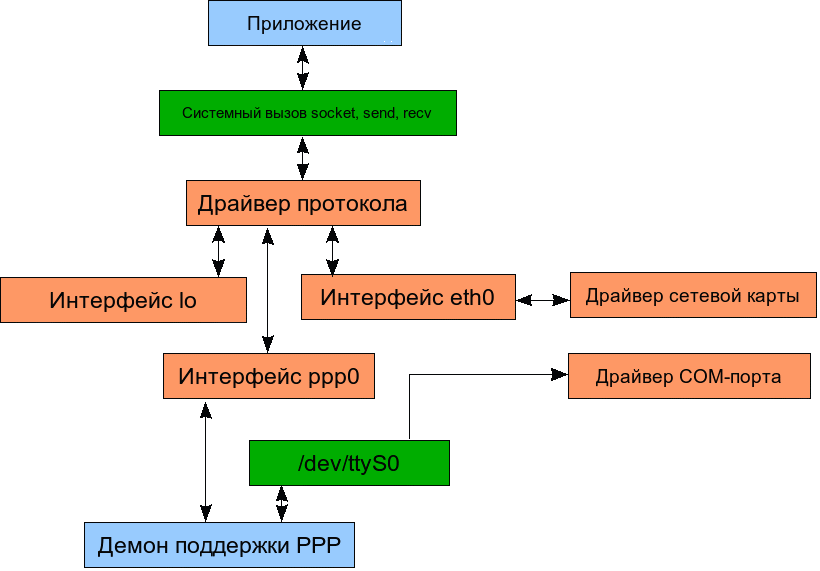
\includegraphics[height=0.8\textheight]{06-netstack.png}

\end{frame}

\begin{frame}{Команды управления настройками сети}
	\begin{itemize}
	  \item ifconfig/route
	  \item iproute2
	\end{itemize}

	\begin{itemize}
		\item Список интерфейсов
			\begin{itemize}
				\item {\tt ifconfig -a}
				\item {\tt ip link show}
			\end{itemize}
		\item Включение интерфейса 
			\begin{itemize}
				\item {\tt ifconfig <iface> up}
				\item {\tt ip link set <iface> up}
			\end{itemize}
	  \item Выключение интерфейса
			\begin{itemize}
				\item {\tt ifconfig <iface> down}
				\item {\tt ip link set <iface> down}
			\end{itemize}
	  \item Назначение адреса
			\begin{itemize}
				\item {\tt ifconfig eth0 192.168.1.17 netmask 255.255.254.0 up}
				\item {\tt ip addr add 192.168.1.17/23 dev eth0}
			\end{itemize}
	\end{itemize}
\end{frame}

\begin{frame}{Конфигурационные файлы}
  \begin{itemize}
    \item {\tt /etc/resolv.conf}
    \item {\tt /etc/hosts}
	\item {\tt /etc/sysconfig/network}
    \item {\tt /etc/sysconfig/network-scripts}\\
		{\tt /etc/sysconfig/network-scripts/ifcfg-eth0}
  \end{itemize}
\end{frame}

\begin{frame}{Дополнительные интерфейсы}
	\begin{block}{Алиасы}
		\begin{itemize}
			\item ifconfig <iface>:<alias> <ip> up
			\item ifconfig <iface> add <ip> up
			\item ip addr add <ip> {\bf label} <iface>:<alias> dev <iface>
		\end{itemize}
	\end{block}
\end{frame}

\begin{frame}{''Виртуальные'' интерфейсы}
	\begin{block}{TUN/TAP}

		{\tt modprobe tun}

		\begin{itemize}
			\item Добавить -- {\tt tunctl -t <ifacename>}
			\item Удалить -- {\tt tunctl -d <ifacename>}
		\end{itemize}
	\end{block}
\end{frame}

\begin{frame}{Мосты}
	\begin{itemize}
		\item Создать -- {\tt brctl addbr <bridge>}
		\item Удалить -- {\tt brctl delbr <bridge>}
		\item Добавить интерфейс -- {\tt brctl addif <bridge> <device>}
		\item Удалить интерфейс-- {\tt brctl addif <bridge> <device>}
	\end{itemize}
\end{frame}

\begin{frame}{Полезные утилиты}

	\begin{itemize}
		\item telnet
		\item netstat / ss
		\item ping
		\item traceroute
		\item tcpdump
		\item nmap
		\item nslookup / dig
	\end{itemize}

\end{frame}

\begin{frame}{Маршрутизация}
	\begin{itemize}
		\item netstat -r
		\item route
		\item ip route show
	\end{itemize}

	\begin{block}{Разрешить маршрутизацию на хосте}
		{\tt echo 1 > /proc/sys/net/ipv4/ip\_forward}
	\end{block}
\end{frame}


\begin{frame}{Iptables}

	\center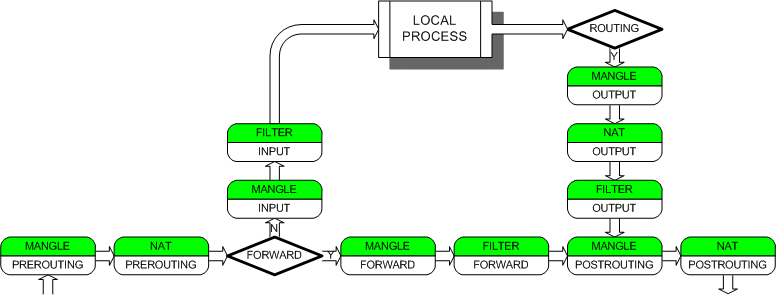
\includegraphics[height=0.4\textheight]{06-iptables.png}

	\begin{itemize}
	\begin{columns}
		\column{0.3\textwidth}
			\item[ ] {\bf iptables -L -t <table>}
				\bigskip

			\item filter -- файерволл
				\begin{itemize}
					\item INPUT
					\item FORWARD
					\item OUTPUT
				\end{itemize}
		\column{0.3\textwidth}
			\item nat -- преобразования адресов
				\begin{itemize}
					\item PREROUTING
					\item INPUT
					\item OUTPUT
					\item POSTROUTING
				\end{itemize}
		\column{0.3\textwidth}
			\item mangle -- специальные  изменения  пакетов (TOS, TTL, MARK)
				\begin{itemize}
					\item PREROUTING
					\item INPUT
					\item FORWARD
					\item OUTPUT
					\item POSTROUTING
				\end{itemize}
		\end{columns}
	\end{itemize}

\end{frame}

\begin{frame}{Практика: создание тестовой среды}
	\begin{itemize}
		\item Подготовка диска
			\begin{itemize}
				\item Создать пустой файл размером в 1GB и отобразить на устройство
					/dev/loop ({\tt dd, losetup})
				\item Создать группу томов на базе этого устройства ({\tt pvcreate, vgcreate})
				\item Выделить 75\% объема под логический диск ({\tt lvcreate})
				\item Скопировать содержимое виртуального диска в полученный логический том ({\tt dd})
				\item Создать снимок логического тома на 20\% размера ({\tt lvcreate})
			\end{itemize}
	\end{itemize}
\end{frame}

\begin{frame}{Практика: создание тестовой среды}
	\begin{itemize}
		\item Запуск виртуальных машин
			\begin{itemize}
				\item {\tt modprobe kvm-intel} 
				\item {\tt modprobe tun} 
				\item {\tt kvm -m 512 -boot c -net nic -net tap,ifname=tap0,script=no,downscript=no /dev/VG0/origin } 
				\item {\tt kvm -m 512 -boot c -net nic -net tap,ifname=tap1,script=no,downscript=no /dev/VG0/snap } 
			\end{itemize}
			\pause
		\item Настройка сети на хосте
			\begin{itemize}
				\item Создать мост {\tt brctl} и назначить ему адрес {\tt ifconfig/ip}
				\item Поднять виртуальные интерфейсы {\tt ifconfig/ip}
				\item Добавить дополнительный интерфейс и виртуальные интерфейсы к мосту {\tt brctl}
			\end{itemize}
			\pause
		\item Настройка сети на виртуалках
			\begin{itemize}
				\item Назначить адрес устройству eth0 {\tt ifconfig/ip}
				\item Проверить {\tt ping}
			\end{itemize}

	\end{itemize}
\end{frame}




\end{document}
